
%% CLASS MANUAL FOUND at http://blog.poormansmath.net/latex-class-for-lecture-notes/ %%
%% CLASS AUTHOR Stefano Maggiolo %%
\documentclass[english,course]{Notes}
%~/Library/texmf/tex/latex/notes.cls

\title{MATHEMATICS 1S}
\subject{Mathematics}
\author{Joao Almeida-Domingues}
\email{2334590D@student.gla.ac.uk}
\speaker{Dr. Andrew Wilson}
\date{07}{01}{2019}
\dateend{24}{05}{2019}
\place{University of Glasgow}

\usepackage[backend=biber, style=reading]{biblatex}
\bibliography{M1Sbiblio}


 %%%%% GENERAL MATHEMATICAL NOTATION SHORTCUTS %%%%%
 
\newcommand{\n}{\mathbb{N}}
\newcommand{\z}{\mathbb{Z}}
\newcommand{\q}{\mathbb{Q}}
\newcommand{\cx}{\mathbb{C}}
\newcommand{\real}{\mathbb{R}}
\newcommand{\field}{\mathbb{F}}
\newcommand{\ita}[1]{\textit{#1}}
\newcommand{\oneton}{\{1,2,3,...,n\}}
\newcommand\ef{\ita{f} }
\newcommand\inv[1]{#1^{-1}}
\newcommand\setb[1]{\{#1\}}
\newcommand\en{\ita{n }}
\newcommand\comb[2]{^{#1}C_{#2}}
\newcommand\perm[2]{^{#1}P_{#2}}

%\renewcommand\qedsymbol{QED} %to use QED instead of square


%%%%%%%%%%%%%%%%PACKAGES%%%%%%%%%%%%%%%%%%%%%%%%%%%%%
\usepackage{lipsum}  
\usepackage{amsmath,amsthm,amssymb,graphicx,mathtools,tikz,pgfplots,minibox} %maths
\pgfplotsset{compat=1.16}
\usepackage{hyperref,framed,color,fancybox} %layout
% framed :  \begin{shaded,frame,snugshade or leftbar} \definecolor{shadecolor}{rgb}{XYZ} to change color
%fancybox: \shadowbox,ovalbox or doublebox
%%%%%%%%%%%%%%%%%%%%%%%%%%%

%%%CLASS SHORTCUTS%%%%
%\lecture{day}{month}{year} for margin note 
%\begin{theorem} sdfsdf\end{theorem} %theo
%\begin{proposition} dfsdfs\end{proposition}
%\begin{lemma} dsfsd \end{lemma} %lem
%\begin{corollary} f ffew \end{corollary}
%\begin{definition} fwewef w \end{definition} %defn
%\begin{example} feww e\end{example} %ex
%\begin{exercise} wefwe \end{exercise}
%\begin{remark} wef we \end{remark} %rem
%\begin{fact} wefe \end{fact}
%\begin{problem} wef ew \end{problem}
%\begin{conjecture} ewfew \end{conjecture}
%\begin{claim} few w \end{claim} 
%\begin{notation} fewf \end{notation} %nota

\begin{document}
\newpage

\section{Vectors}

\subsection{Generalities}

\lecture{07}{01}{2019}

\defn{A scalar}{is a one-component quantity that is invariant under rotations of the coordinate system, which describes the magnitude of something}

\defn{A vector}{ is a two-component quantity, with magnitude (a positive real number) and direction}

\rem{If a vector has both a magnitude and direction of $0$, then that vector is  the zero vector. The zero vector can be thought as having no direction, or all directions}

\defn{Equality:}{ Two vectors are equal if they have the same magnitude and the same direction\label{def:eq}}

\rem{Every vector is unique}

\proofs{ Let $\vc{u}, \vc{v}$ be two vectors with magnitude $\lambda$ and the same direction. Hence by \ref{def:eq} , $\vc{u} = \vc{v}$}


\nota{ Generally, in printed text $\overrightarrow{v} \text{ or } \ \vc{v}$. Handwritten \underline{$v$}. Magnitude $\vc{|v|}$}

\defn{Unit vector}{is a vector of magnitude 1. There is exactly one for any given direction}
\nota{Generally, for a given vector $\vc{v} \ , \ \hat{\vc{v}}$}

\prop{Parallelogram }{$\overrightarrow{AB} = \overrightarrow{DC}$\ , i.e Traversing left-up is the same as up-right}
\proofs{It follows from the fact that the opposite sides of a parallelogram are parallel and of equal length. Hence they are equal, by \ref{def:eq}}

\prop{Negative vectors }{$\overrightarrow{AB} = u \iff \overrightarrow{BA} = -u$}
\proofs{It follows from the fact that they have the same magnitude but opposite directions}

\prop{Zero vector }{$\overrightarrow{AA} = 0$}
\proofs{For any point $A, |AA| = 0$ and so $\overrightarrow{AA} = 0$}

\subsection{Addition and Scalar Multiplication}

\defn{Addition}{Let $\vc{u} = \overrightarrow{PQ} \ , \ \vc{v} = \overrightarrow{QR}. \vc{u} + \vc{v} = \overrightarrow{PR}$. \ita{nose-to-tail}}

\rem{As per usual subtraction is simply, $\vc{u} + (-\vc{v})$}

\defn{Scalar Multiplication}{For a vector $\vc{u}$, and a scalar $\lambda$. $\lambda\vc{u}$ scales the vector's magnitude  by $\lambda$, and if $\lambda<0$ inverts its direction}

\lecture{8}{01}{2019}
\subsubsection{Properties of Addition and Multiplication}
\prop{Commutative }{$\vc{u} + \vc{v} = \vc{v} + \vc{u}$}
\proofs{
\begin{align*}
	 \vc{u} + \vc{v} & = [u_1, u_2 , \dots , u_n] + [v_1 , v_2 , \dots , u_n] \\
	 & = [u_1 + v_1 , u_2 + v_2 , \dots , u_n + v_n] \text{  \ita{vector addition}} \\
	 & = [v_1 + u_1, v_2 + u_2 , \dots , v_n + u_n] \text{  \ita{commutative adition of real numbers}} \\
	 & = [v_1 , v_2 , \dots , v_n] + [u_1, u_2 , \dots , u_n] \\
	 & = \vc{v} + \vc{u}
\end{align*}
}


\prop{Associative }{$(\vc{u} + \vc{v}) + \vc{w} = \vc{u} + (\vc{v} + \vc{w})$}
\proofs{
\begin{align*}
	(\vc{u} + \vc{v}) + \vc{w} & = ([u_1, u_2 , \dots , u_n] + [v_1 , v_2 , \dots , v_n]) + [w_1 , w_2 , \dots , w_n] \\
	 & = [u_1 + v_1 , u_2 + v_2 , \dots , u_n + v_n]  + [w_1 , w_2 , \dots , w_n]   \mathbf(1.10) \\
	 & = [(u_1 + v_1) + w_1, (u_2 + v_2) + w_2, \dots , (u_n + v_n) + w_n] \text{  \ita{commutative property of scalars}} \\
	 & = [u_1 + (v_1 + w_1), u_2 + ( v_2 + w_2), \dots , u_n + (v_n + w_n)] \text{  \ita{associative addition of real numbers}} \\
	 & = [u_1 , u_2 , \dots , u_n] + [v_1 + w_1 , v_2 + w_2 , \dots , v_n + w_n]  \\
	 & = \vc{u} + \vc{v} + \vc{w}
\end{align*}
}

\prop{Distributive }{$\lambda(\vc{u} + \vc{v}) = \lambda\vc{u} +\lambda\vc{v}$}
\proofs{
\begin{align*}
	\lambda(\vc{u} + \vc{v}) & = \lambda([u_1 + v_1 , u_2 + v_2 , \dots , u_n + v_n])   \text{  \ita{vector addition}} \\ 
	& = [\lambda(u_1 + v_1) , \lambda(u_2 + v_2) , \dots , \lambda(u_n + v_n)] \text{  \ita{scalar multiplication} }\\
	& = [\lambda u_1 + \lambda v_1 , \lambda u_2 + \lambda v_2 , \dots , \lambda u_n + \lambda v_n] \text{  \ita{distributive for real numbers}} \\
	& = \lambda\vc{u} + \lambda\vc{v}
\end{align*}
}

\newpage
\proofs{ \ita{2 , by a diagram} \\

Let $\vc{u} , \vc{v}$ be two non-zero vectors, and A, B, C be 3 distinct points. Then:

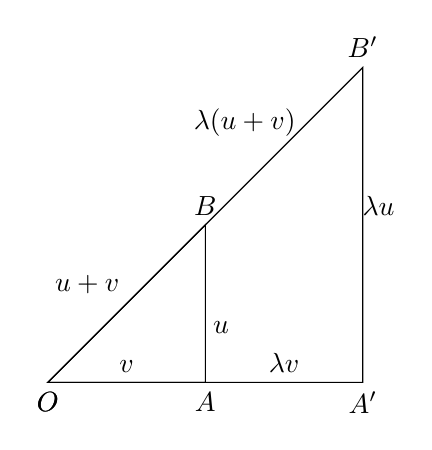
\begin{tikzpicture}
\centering
\draw (0,0) node[anchor=north]{$O$}
  -- (2,0) node[anchor=north]{$A$}
  -- (2,2) node[anchor=south]{$B$}
    -- cycle;
    \draw
  -- (0.5,1) node[anchor=south]{$\vc{u} + \vc{v}$}
  -- (2.2,0.5) node[anchor=south]{$\vc{u}$}
  -- (1,0) node[anchor=south]{$\vc{v}$};


\draw (0,0) node[anchor=north]{$O$}
  -- (4,0) node[anchor=north]{$A'$}
  -- (4,4) node[anchor=south]{$B'$}
  -- cycle;
  \draw
    -- (2.5,3) node[anchor=south]{$\lambda(\vc{u} + \vc{v})$}
  -- (4.2,2) node[anchor=south]{$\lambda\vc{u}$}
  -- (3,0) node[anchor=south]{$\lambda\vc{v}$};
  \end{tikzpicture}

Let the "prime" triangle represent a $\lambda$ fold enlargement of the original triangle representing the original vectors and their addition. Hence we have that,

\begin{align*}
OB' = \lambda(\vc{u} + \vc{v}) & = OA' + A'B' \\
& = \lambda\vc{v} + \lambda\vc{u}
\end{align*}
}







\subsection{Parallel and Position vectors}

\defn{Parallel:}{ Let $\vc{u} \ , \ \vc{v}$ be two non-zero vectors. Then, 
$\vc{v}$ is parallel to $\vc{u}$ \ita{iff} $\vc{v} = \lambda\vc{u}$ (i.e. if they share the same or opposite directions) and $\hat{\vc{u}} = \frac{1}{|\vc{u}|}\vc{u}$}

\nota{$\vc{u} \parallel \vc{v}$}

\rem{The non-zero vector is parallel to all vectors}

\proofs{ The first part of the definition is self-evident as any scalar multiple of a vector will only alter its magnitude and/or reverse its direction. For the second part, we have that:

$$ \bigg|\frac{1}{|\vc{u}|}\vc{u}\bigg| = \frac{1}{|\vc{u}|}|\vc{u}| = 1 $$

Hence, we've shown that $\frac{1}{|\vc{u}|}|\vc{u}|$ is a unit vector of $\vc{u}$, which means that it only varies in magnitude, and is therefore parallel.
}

\defn{Position:}{Let $O$ denote the origin, the vector from $O$ to any point $P$ ($\overrightarrow{OP}$) is called the position vector. For any points  $A \text{ and } B , \overrightarrow{ AB } = \vc{b} -  \vc{a}$}

\nota{ $\vc{r}_p$}

\proofs{ \\

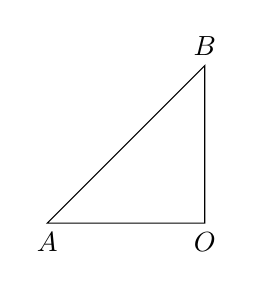
\begin{tikzpicture}
\centering
\draw (0,0) node[anchor=north]{$A$}
  -- (2,0) node[anchor=north]{$O$}
  -- (2,2) node[anchor=south]{$B$}
  -- cycle;
\end{tikzpicture} 
\ \ \ \ \ \  $
\begin{aligned} \overrightarrow{ A B } & = \overrightarrow { A O } + \overrightarrow { O B } \\ & = ( - \mathbf { a } ) + \mathbf { b } \\ & = \mathbf { b } - \mathbf { a } \end{aligned}$
}

\lecture{09}{01}{2019}
\subsection{Collinearity and the section formula}

\defn{Collinear}{points lie on a straight line}

\rem{One can test wether points are collinear by finding if their directed line segments, i.e. the vector formed starting at a point and ending at the other, are parallel.}

\ex{ Let $\overrightarrow{AB} = \vc{u} , \overrightarrow{BC} = 2\vc{u} , \overrightarrow{AC} = \vc{u} + \vc{2u} = \vc{3u}$. Hence they are all parallel to $\vc{u}$, it follows then that they are collinear.}

\rem{ $$ AB : BC = \beta : \alpha \implies \alpha \overrightarrow{AB} = \overrightarrow{BC} $$ }

Setting $\lambda = \frac{\beta}{\alpha}$,

$$ \overrightarrow{AB} = \lambda\overrightarrow{BC} \ \ \ AB : BC = \lambda : 1 $$

\par{Since $A , B \text{ and } C$ are collinear, we can deduce the distance between the points using their ratio \Big($\lambda = \tfrac{|AB|}{|BC|}$\Big). Furthermore, for $\lambda > 0 $ we have that the vectors have the same direction,  hence $B$ lies between $A$ and $C$. Note however that this is not true for $\lambda < 0$} 


\begin{tikzpicture}
\draw (0,0) node[anchor=north]{$A$}
  -- (2,0) node[anchor=north]{$B$}
  node[pos=0.5]{$>$}
  -- (5,0) node[anchor=north]{$C$}
    node[pos=0.5]{$>$}
  	(6,0) node[anchor=north]{$A$}
  -- (8,0) node[anchor=north]{$C$}
  node[pos=0.5]{$>$}
  node[pos=1.5]{$<$}
  -- (10,0) node[anchor=north]{$B$};
   
\end{tikzpicture} x

\prop{Section Formula \label{secForm}}{ Let $A, B \text{ and } P$ be collinear points, s.t:

$$ AP : PB = m : n $$

Then, $P$ has position vector $$ \vc{p} = \frac{m\vc{b} + n\vc{a}}{m + n} $$

\begin{tikzpicture}
\draw (2,0) -- (10,0)
(4,0) node[anchor=north]{$A$}
(5,0) node[anchor=south]{$m$}
(7,0) node[anchor=north]{$P$}
(8,0) node[anchor=south]{$n$}
(9,0) node[anchor=north]{$B$};

\end{tikzpicture}
 }

\proofs{ 
\begin{align*}
n\overrightarrow{AP} &= m \overrightarrow{PB} \\
n(\vc{p} - \vc{a}) &= m(\vc{b} -\vc{p}) \\
(m+n)\vc{p} &= m\vc{b} + n\vc{a} \\
\vc{p} &= \frac{m\vc{b} + n\vc{a}}{m + n}
\end{align*}}

\begin{corollary}{The midpoint of $AB$ has position vector $\tfrac{1}{2}(\vc{a} + \vc{b})$ \mymarginpar{special case of \ref{secForm}, where $m = n = 1$}}\end{corollary}


\mymarginpar{TODO: Applications of  the section formula}


\lecture{14}{01}{19}
\subsection{Scalar/Dot Product}

\defn{Scalar Product}{ of two unit vectors is the cosine of the angle between them. We obtain the scalar product of any two non-zero, non-unit vectors by scaling them by their magnitudes.}

\nota{$ \vc{u} \cdot \vc{v}$}

$$ \hat{\vc{u}} \cdot \hat{\vc{v}} = \cos\theta \ \ \ \& \ \ \  \vc{u} \cdot \vc{v} = |\vc{u}| |\vc{v}| \cos\theta $$

\rem{Note that $\theta \in [0,\pi]$}

\rem{If one of the vectors is a zero vector their scalar product is $0$}

\prop{For any vector $\vc{u}$: $$ \vc{u} \cdot \vc{u} = |u|^2$$}

\proofs{ It follows from the fact that $\theta = 0 , \cos\theta = 1$. Hence: 
	$$  \vc{u} \cdot \vc{u} = |\vc{u}| |\vc{u}| (1) =  |u|^2 $$}

\prop{Two non-zero vectors are perpendicular if their scalar product is $0$}

\proofs{ $\vc{u} \bot \vc{v} \iff \theta = \tfrac{\pi}{2}$. Hence, $\cos\theta = 0$. Therefore: \\

$ \vc{u} \cdot \vc{v} = |\vc{u}| |\vc{v}| (0) = 0$}

\newpage\subsubsection{Properties of Scalar Products}

\prop{Commutative }{$\vc{u} + \vc{v} = \vc{v} + \vc{u}$}

\proofs{ 
\begin{align*}
\vc{u} \cdot \vc{v} &= u_1v_1 + u_2v_2 + \dots + u_nv_n \\
&= v_1u_1 + v_2u_2 + \dots + v_nu_n \ \ \ita{(commutative multiplication of real numbers)}\\
&= \vc{v}\cdot\vc{u}
\end{align*}}

\prop{Distributive  }{ $\vc { u } \cdot ( \vc { v } + \vc { w } ) = \vc { u } \cdot \vc { v } + \vc { u } \cdot \vc { w }$}

\proofs{
\begin{align*}
\vc{u} \cdot (\vc{v} + \vc{w}) &= (u_1,u_2,\cdots,u_n) \cdot (v_1+w_1 , v_2+w_2 , \dots , v_n+w_n) \ \ \ita{(vector addition)} \\
&= u_1(v_1+w_1) + u_2(v_2+w_2) + \dots +  u_n(v_n+w_n) \ \  \ita{(vector multiplication)} \\
&= (u_1v_1 + u_1w_1) + (u_2v_2 + u_2w_2) + \dots +  (u_nv_n + u_nw_n) \ \ \ita{(scalar multiplication)} \\
&= (u_1v_1 + u_2v_2 + \dots + u_nv_n) + (u_1w_1 + u_2w_2 + \dots + u_nw_n) \ \ \ita{(associativity of real numbers)} \\
&= \vc{u}\vc{v} + \vc{u}\vc{w}
\end{align*}
}

\prop{NON-Associative}{}
\proofs{$\vc{u} \cdot (\vc{v} \cdot \vc{w})$ is an invalid expression, since the dot product returns a scalar and we cannot perform the dot product between a scalar and a vector}

\subsection{Normal to a Plane}

\defn{A normal to a plane}{ is a vector that is at right-angles to every vector contained within it}

\rem{Every plane has two normals, one pointing "upwards" and another "downwards"}

\rem{Note that there are infinitely many planes, lying parallel to one another~\mymarginpar{Think of stack}. Hence, to define a plane one needs to know its normal and a point within it.}

\defn{Plane~\label{vectors:plane}}{We observe that a point p lies on P, given a normal $\vc{n}$, \ita{iff} the dot product between the directed line segment on the plane and the normal is $0$.  $$ P = \text{\{points P } |  \ \vc{n} \cdot \overrightarrow{pP} = 0 \} \label{plane:normal} $$}

\newpage
\lecture{15}{01}{2019}

\subsection{Cross Product}

\par{To start exploring the nature of the cross product of two 3D vectors, we first note that the two vectors form an area. We see this often exemplified by the parallelogram rule. Now let $A(\theta)$ represent the area demarcated by this parallelogram. This function of $\theta$ has its maximum when $\theta = \tfrac{\pi}{2}$ , i.e. when the parallelogram is a square, and its minimum when $\theta =  0$ , i.e. $\vc{u}$ and $\vc{v}$ are parallel.}

$$A ( \theta ) = \left\{ \begin{array} { l l } { 0 } & { \text { when } \theta = 0 } \\ { | \mathbf { u } | | \mathbf { v } | } & { \text { when } \theta = \frac { \pi } { 2 } } \\ { 0 } & { \text { when } \theta = \pi } \end{array} \right.$$

\defn{Cross Product}{$\vc{u} \times \vc{v}$ is a vector with magnitude $|\vc{u}||\vc{v}|\sin\theta$*\mymarginpar{*this is just the area of the parallelogram} and direction given by the normal~\ref{cross:rhr} of the plane on which the parallelogram lies}

\defn{Righ-Hand Rule~\label{cross:rhr}}{Convention used to fix the direction of the parallelogram uniquely \scriptsize{(remember that this is because it could point "upwards" or "downwards")}. \normalsize By putting the index finger parallel to the palm, and orientating the thumb and first finger in the directions of $\vc{u} , \vc{v}$. The index finger gives us the fixed direction}



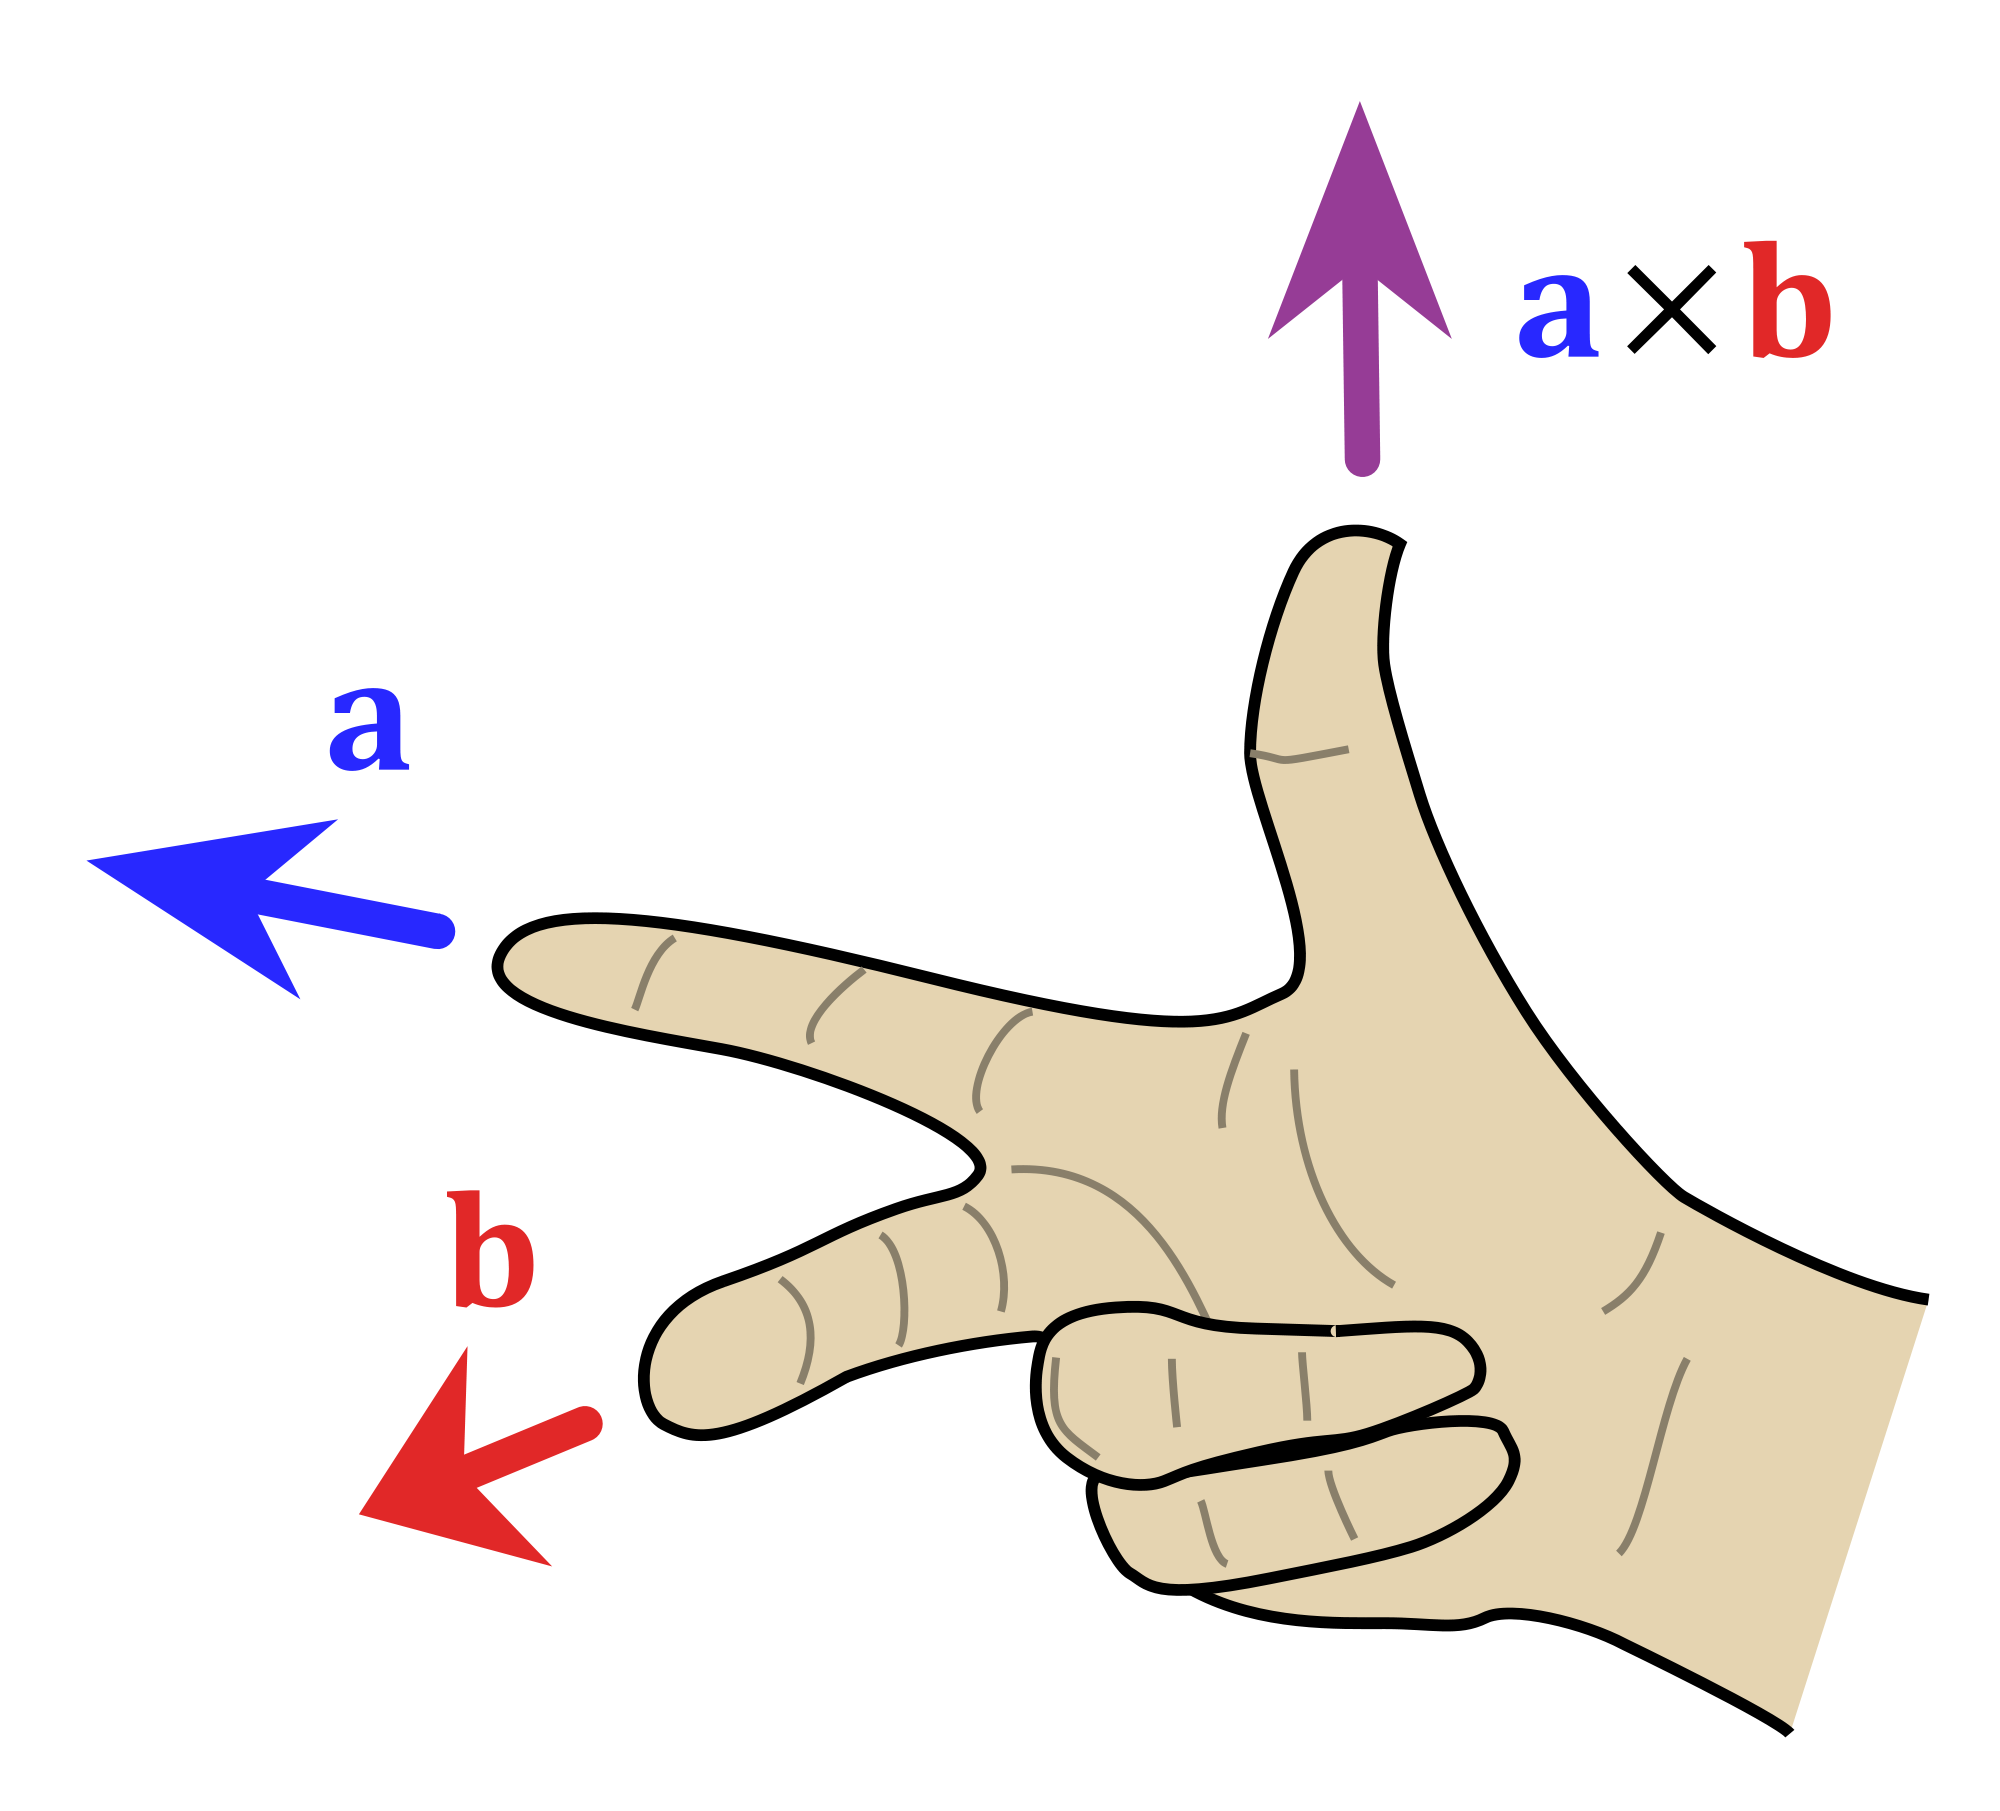
\includegraphics[width=0.3\textwidth]{assets/hand}



\prop{Parallelism Criterion}{ Two non-zero vectors are parallel \ita{iff}  \\ $ \vc{u} \times \vc{v} = 0$}

\proofs{This follows from the fact that two vectors are parallel if $\theta = 0$ or $\theta = \pi$ , either way $\sin\theta = 0$ , therefore $|\vc{u}||\vc{v}|\sin\theta = 0$}

\rem{Note how for the dot product we start by looking at the parallelism of two vectors, and get a criterion for their perpendicularity. Whilst for the cross product the opposite is true.}

\subsubsection{Properties of the Cross Product}

\rem{Note that the cross product is only valid up to 3D}

\prop{Anti-Commutative}{\ \ \ $\vc{a} \times \vc{b} \neq \vc{b} \times \vc{a}$ $$\vc{a} \times \vc{b} = - \vc{b} \times \vc{a}$$}

\proofs{For non-parallel vectors, the result follows from the fact that even though the magnitude remains unchanged*~\mymarginpar{*just like in the dot product} , i.e. $|\vc{u} \times \vc{v}| = |\vc{v} \times \vc{u}| = |\vc{u}||\vc{v}|\sin\theta$, their direction is reversed.}

\prop{NON-Associative}{}
\proofs{ Let $\vc{a}$ and $\vc{v}$ be two distinct non-zero vectors. Then we have:

\begin{align}
&\vc{a} \times (\vc{a} \times \vc{c}) \neq 0~\label{assoc:1} \\ 
&\underbrace{(\vc{a} \times \vc{a})}_{\ita{\scriptsize $0$ , since $\theta = 0$}}   \times \vc{c} = 0~\label{assoc:2}
\end{align}

\eqref{assoc:1} and \eqref{assoc:2} cannot both be true, hence we arrive at a contradiction.}

\prop{Distributive across scalar multiplication and addition}{}
\mymarginpar{addition proof beyond 1S's scope}

\proofs{ \\
$$\lambda (\vc{a} \times \vc{b}) = |\lambda\vc{a} \times \vc{b}| = |\vc{a} \times \lambda\vc{b}|$$
$$\vc{c}(\vc{a} + \vc{b}) = \vc{c} \times \vc{a} + \vc{c} \times \vc{b}$$}

\rem{Note that the dot and cross product do not distribute amongst themselves}
\proofs{ \begin{align}
& (\vc{a} \times \vc{b}) \cdot \vc{c}\ \ \  \ita{ Valid} \\
& \underbrace{(\vc{a} \cdot \vc{b})}_{\ita{yields a scalar}} \times \vc{c} \ \ \ \ita{ Invalid, scalar $\times$ vector not allowed}
\end{align}
}

\textbf{Application of the Cross Product}
\lecture{21}{01}{2019}
\ex{
\par{Three points A, B and C determine the plane P containing them. Find a criterion for a point P to lie on P in terms of A, B and C. \\ }

\par{It follows from (\ref{vectors:plane}), that we need to find the normal $n$ to the plane containing $A, B
\text{ and }C$. And given that $\overrightarrow{AB}$ and $\overrightarrow{AC}$ lie in $P$:}

$$\vc{n} = \overrightarrow{AB} \times \overrightarrow{AC}$$

\par{So the criterion is: $\overrightarrow{AP} \times \cdot \vc{n} = \overrightarrow{AP} \cdot (\overrightarrow{AB} \times \overrightarrow{AC}) = 0$}
}

\newpage

\section{Counting Methods}

\subsection{The Multiplication Principle}

\defn{Multiplication Principle}{Let the joint experiment $ \theta $, represent an experiment, with $k$ possible outcomes, composed by two other distinct experiments $\lambda_1$ and $\lambda_2$ each witch $n_1$ and $n_2$ possible outcomes, respectively. Then, $k = n_1 \cdot n_2$}

\subsection{Combinations and Permutations}
\defn{Combinations}{For a collection of $n$ different objects, by selecting $r$ of them, the number of possible combinations where the \textbf{order does not matter}  is given by: \mymarginpar{Note the similarity of the formulas, since the order is irrelevant, we should expect the possible \# of combinations to decrease, hence higher denominator}
$$ {n \choose r} = \ \comb{n}{r} = \frac{n!}{(n-r)!r!}$$}

\defn{Permutations}{For a collection of $n$ different objects and $n$ spaces, the number of permutations is the number of possible ordered arrangements. It is given by $n!$}

\nota{More generally, when only wishing to select an $r$ number of those $n$ objects, where $0 \leq r \leq n$: $$\perm{n}{r} = \frac{n!}{(n-r)!}$$}

\rem{More generally still, for repeated objects ($n_1$ of type 1, \dots, $ n_t $ of type $t$): $$ \frac{n!}{n_1!
\times \dots \times n_t!}$$}

\lecture{22}{01}{2019}
\par{Note that we can obtain the permutations formula by looking at forming permutations of $r$ objects from
$n$ as a two stage procedure:}

\begin{enumerate}
	\item Choose any combination of $r$ objects: $\comb{n}{r}$
	\item Order the $r$ objects: $r!$
\end{enumerate}

\textbf{Properties of $n \choose r$}

\prop{ For $n \in \n$ and $ r = 0,1,\dots$: $$ { n \choose n-r} = {n \choose r}$$~\label{choose:1}}

\proofs{ \begin{align*}
{n \choose n-r} & = \frac{n!}{(n-(n-r))!(n-r)! } \\ & = \frac{n!}{r! (n-r)!} \\ & = {n \choose r}
\end{align*}}

\ex{Determine, as efficiently as possible, the following:

$$ {n \choose 0} , {n \choose 1} , {n \choose 2} , {n \choose 3} , {n \choose 4} , {n \choose 5}\\ $$

\par{By using the symmetry which follows from (\ref{choose:1}) we have that:}

$$ {n \choose 0} = {n \choose 5} = 1 \ ; \ {n \choose 1} = {n \choose 4 } = 5 \ ; \ {n \choose 2} = {n \choose 3} = 10 $$
}


\subsection{Combinations subject to Constraints}

\begin{enumerate}
	\item Exclusion of $k$ objects: $${n \choose r}\bigg| _{\text{exclude }k} = {n-k \choose r}$$	
	\item Inclusion of $k$ objects: $${n \choose r}\bigg|_{\text{include }k} = {n-k \choose r-k}$$
	\item Complement: The number of combinations that do satisfy a constraint is the complement of the number that do not $$ \text{Combinations which satisfy the constraint } = \text{Total - Combinations which do not }$$
\end{enumerate}

\newpage	
\subsection{Pascal's Triangle}
\lecture{28}{01}{2019}

\par{The pascal's triangle is formed by setting the edges to $1$, and generating numbers for each row by summing the two numbers immediately above them. So that, for each row $n$, each entry represents choosing $n$ objects from $ 0 \to n$ }

$$
\begin{tabular}{rccccccccccccc}
$n=0$:&    &    &    &    &    &    &  1\\\noalign{\smallskip\smallskip}
$n=1$:&    &    &    &    &    &  1 &    &  1\\\noalign{\smallskip\smallskip}
$n=2$:&    &    &    &    &  1 &    &  2 &    &  1\\\noalign{\smallskip\smallskip}
$n=3$:&    &    &    &  1 &    &  3 &    &  3 &    &  1\\\noalign{\smallskip\smallskip}
$n=4$:&    &    &  1 &    &  4 &    &  6 &    &  4 &    &  1\\\noalign{\smallskip\smallskip}
$n=5$:&    &  1 &    &  5 &    & 10 &    & 10 &    &  5 &    &  1\\\noalign{\smallskip\smallskip}
$n=6$:&  1 &    &  6 &    & 15 &    & 20 &    & 15 &    &  6 &    &  1\\\noalign{\smallskip\smallskip}
\end{tabular}$$

\par{This construction relies on the following:}
 
\prop{For $n \in \n \text{ and } r = 1, 2, . . . , n,$ $$ {n+1 \choose r} = {n \choose r-1} + {n \choose r}$$}

\proofs{}
\mymarginpar{TODO: enquire about the exclusion bit of the proof}

\lecture{29}{01}{2019}

\subsection{Binomial Theorem}

\par{Note that when expanding polynomials of the type $(a + b)^n$, we obtain a
number of factors which are $a$ and a certain number which are $b$ with
the total number of factor always equal to $n$ terms of the following form:

$$a ^ { n } , a ^ { n - 1 } b , a ^ { n - 2 } b ^ { 2 } , \dots , a ^ { 2 } b ^ { n - 2 } , a b ^ { n - 1 } , b ^ { n }$$

If we let $r$ be a $0$-based index, then more generally, a term at position $r$ is given by:

$$r = a^{n-r}b^r$$}

\par{Using our knowledge of combinatorics we can calculate the number of times each term appears in the expanded expression , i.e. their \ita{binomial coefficients}}

$${n \choose 0} a ^ { n } , {n \choose 1} a ^ { n - 1 } b , {n \choose 2} a ^ { n - 2 } b ^ { 2 } , \dots , {n \choose {n-2}} a ^ { 2 } b ^ { n - 2 } , {n \choose {n-1}} a b ^ { n - 1 } , {n \choose {n}} b ^ { n }$$


\theo{$$( a + b ) ^ { n } = \sum _ { r = 0 } ^ { n } { n \choose r} a ^ { n - r } b ^ { r }$$} 




\begin{corollary}

$$(a-b)^n = (a+(-b))^n = \sum_{r=0}^n {n \choose r} a^{n-r}(-b)^r$$

\end{corollary}

\rem{the signs alternate between even and odd powers of $b$}

\begin{corollary}

$$(1+x)^n = \sum_{r=0}^n {n \choose r}x^r$$

\end{corollary}

\subsection{Applications to Trigonometry}
\lecture{04}{02}{2019}
\subsubsection{1}
\par{Applying the binomial theorem in conjunction with de Moivre's we can write $\cos(n\theta)$ and $\sin(n\theta)$ in terms of $\cos(\theta)$ and $\sin(\theta)$.}

\ex{ Express $\cos(5\theta)$ as a polynomial in $\cos(\theta)$ and $\sin(5\theta)$ as a polynomial in $\sin(\theta)$\\
\par{Let $\cos(\theta) = c$ and $\sin(\theta) = s$}

\begin{align*}
	\cos(5\theta) + i\sin(5\theta) &= (c + is)^5 \quad \ita{de Moivre's} \\
	&= c ^ { 5 } + 5 c ^ { 4 } ( i s ) + 10 c ^ { 3 } ( i s ) ^ { 2 } + 10 c ^ { 2 } ( i s ) ^ { 3 } + 5 c ( i s ) ^ { 4 } + ( i s ) ^ { 5 } \ita{  Binomial Theorem}\\
	&= c ^ { 5 } + i \left( 5 c ^ { 4 } s \right) - 10 c ^ { 3 } s ^ { 2 } - i \left( 10 c ^ { 2 } s ^ { 3 } \right) + 5 c s ^ { 4 } + i s ^ { 5 } \\
	&= c ^ { 5 } - 10 c ^ { 3 } s ^ { 2 } + 5 c s ^ { 4 } + i \left( 5 c ^ { 4 } s - 10 c ^ { 2 } s ^ { 3 } + s ^ { 5 } \right)
\end{align*}


\par{Equating the real parts:}

\begin{align*}
	\cos(5\theta) &= c^5 - 10c^3s^2 + 5cs^4 \\
		&= c^5 - 10c^3(1-c^2) + 5c(1-c^2)^2 \\
		&= c^5 - 10c^3 + 10c65 + 5c - 10c^3 + 5c^5 \\
		&= \boxed{16\cos^5(\theta) - 20\cos^3(\theta) + 5\cos(\theta)}
\end{align*}
\newpage
\par{Equating the imaginary parts:}

\begin{align*}
\sin(5\theta) &=  5 c ^ { 4 } s - 10 c ^ { 2 } s ^ { 3 } + s ^ { 5 }  \\ 
&= 5 \left( 1 - s ^ { 2 } \right) ^ { 2 } s - 10 \left( 1 - s ^ { 2 } \right) s ^ { 3 } + s ^ { 5 }  \\ 
&=  5 s - 10 s ^ { 3 } + 5 s ^ { 5 } - 10 s ^ { 3 } + 10 s ^ { 5 } + s ^ { 5 } \\ 
&=  \boxed{16 \sin ^ { 5 } \theta - 20 \sin ^ { 3 } \theta + 5 \sin \theta}
\end{align*}
}
 
 \subsubsection{2}
 
 \par{Conversely, let $z= e^{ir\theta}$. Note that,
 
 $$e^{i\theta} + e^{-i\theta} = \cos(\theta) + \cancel{\sin(\theta)} + \cos(\theta) - \cancel{\sin(\theta)} = 2\cos(\theta) \iff \boxed{\cos(r\theta) = \frac{1}{2}(z^{r} + z^{-r})}$$
 
$$e^{i\theta} - e^{-i\theta} = \cancel{\cos(\theta)} + \sin(\theta) - \cancel{\cos(\theta)} + \sin(\theta) = 2i\sin(\theta) \iff \boxed{\sin(r\theta) = \frac{1}{2i}(z^{r} - z^{-r})}$$
}

\ex{Express $\cos^6{\theta}$ in the form $a \cos^6(\theta) + b \cos^4(\theta) + c \cos^2(\theta) + d$\\

\par{Using the binomial theorem, and the formulae above with $2\cos(\theta)$ so that we get rid of the fraction during the working out we have that:}

\begin{align*}
(2\cos(\theta))^{6} &= (z + z^{-1})^6 \\
	&= z ^ { 6 } + 6 z ^ { 5 } z ^ { - 1 } + 15 z ^ { 4 } z ^ { - 2 } + 20 z ^ { 3 } z ^ { - 3 } + 15 z ^ { 2 } z ^ { - 4 } + 6 z z ^ { - 5 } + z ^ { - 6 } \\
	&=  z ^ { 6 } + 6 z ^ { 4 } + 15 z ^ { 2 } + 20 + 15 z ^ { - 2 } + 6 z ^ { - 4 } + z ^ { - 6 }  \\ 
	&= \left( z ^ { 6 } + z ^ { - 6 } \right) + 6 \left( z ^ { 4 } + z ^ { - 4 } \right) + 15 \left( z ^ { 2 } + z ^ { - 2 } \right) + 20  \\ 
	&=  2 \cos ( 6 \theta ) + 12 \cos ( 4 \theta ) + 30 \cos ( 2 \theta ) + 20 
\end{align*}

\begin{align*}
\iff \cos^6(\theta) &= \frac{1}{64}\left(2 \cos ( 6 \theta ) + 12 \cos ( 4 \theta ) + 30 \cos ( 2 \theta ) + 20 \right)
\end{align*}

}
%%%%%%%%%%%%%%%%%%%%%%%
\newpage
\section{Coordinates \& 3D Geometry}
\lecture{05}{02}{2019}

\subsection{Standard Unit Vectors}

\par{We represent the unit vectors with the same direction as the $x, y, z$ axes by $\vc{i} , \vc{j} , \vc{k}$ respectively. And we can represent any position vector by combining multiples of these (~\ref{3d:comp})}

\nota{$P(\alpha, \beta, \lambda)$ represents an arbitrary point}

\nota{$P = (\alpha, \beta, \lambda)$ represents an arbitrary vector}

\par{So we have that $$ \vc{i} = (1,0,0) \quad \vc{j} = (0,1,0) \quad  \vc{k} = (0,0,1)$$}

\prop{}{$$\vc{r}_p = \alpha\vc{i} + \beta\vc{j} + \lambda\vc{k}$$

\par{and}

$$|\vc{r}_p|^2 = \alpha^2 + \beta^2 + \lambda^2$$
}

\proofs{ (see figure 3.4 lecture notes)}

\prop{Distance Formula~\label{3d:distance}}{ For two points $A(x,y,z), B(m,n,o)$

$$|AB| = \sqrt{(m-x)^2 + (n-y)^2 + (z-o)^2}$$
}

\proofs{Follows from above, where $A$ is not the origin $(0,0,0)$}

\subsection{Vector Products}

\par{By noting that the standard unit vectors are at an angle of $\frac{\pi}{2}$ it follows that 

$$ |\vc{i} \times \vc{j}| = |\vc{i}| |\vc{j}| \sin\left(\frac{\pi}{2}\right) = 1$$

and by the rhr (~\ref{cross:rhr}) we also note that $ \vc{i} \times \vc{j} = \vc{k}$
}

\defn{Right-Handed System}{We call the \ita{triple} $(\vc{i},\vc{j},\vc{k})$ a rhs of vectors}

\par{There are two easy ways to see if a rotation of $(\vc{i},\vc{j},\vc{k})$ is still a valid rhs. (1) make sure that all the positive axis are facing "your way" (2) using a circular diagram with i at the top, taking the positive , and hence valid, rotations to be anti-clock wise. So we have other two valid permutations which originate a rhs $(\vc{j}, \vc{k}, \vc{i}) , (\vc{k}, \vc{i}, \vc{j})$}

\rem{lhs results in negative angles, hence negative products}

\prop{}{ Let $\vc{i}, \vc{j}, \vc{k} $ be the standard unit vectors, then:

$$\vc{i} \times \vc{j} = \vc{k} \quad \vc{j} \times \vc{k} = \vc{i} \quad \vc{k} \times \vc{i} = \vc{j}$$

and

$$\vc{k} \times \vc{j} = -\vc{i} \quad \vc{j} \times \vc{i} = \vc{k} \quad \vc{i} \times \vc{k} = \vc{j}$$
}

\subsection{Component Form}

\defn{Component Form~\label{3d:comp}}{ vector represented in terms of $\vc{i} , \vc{j}, \vc{k}$. For a given point $P(\alpha, \beta, \lambda)$

$$ \vc{u} = \alpha\vc{i} + \beta\vc{j} + \lambda\vc{k}$$
}

We can rewrite (\ref{3d:distance}) in terms of $(\alpha, \beta, \lambda)$

\prop{}{For $\vc{u} = (\alpha, \beta, \lambda)$

$$|\vc{u}| = \sqrt{\alpha^2 + \beta^2 + \lambda^2}$$
}

\lecture{11}{02}{2019}

\subsection{Section Formula in Component Form}

\ex{ 

$$ \text{Points: } A ( 3 , - 2,4 ) , B ( 4,0,2 ) , C ( 7,6 , - 4 ) , D ( 1 , - 7,0 ) $$
\begin{itemize}
\item[a] Are $ A , B , D$ collinear? If so, find $A B : B D$ 
\item[b] Find the point $P$ on $AC$ such that $ A P : P C = - 1 : 5 $ 
\end{itemize}

\par{ Note that the position vectors are given by the coordinates of the points, it follows then:}
\begin{itemize}
\item[a]

$$AB = \vc{b} - \vc{a} = (1, 2, -2) \quad BD = \vc{d} - \vc{b} = (-2, -7, -2)$$

\par{Given that the vectors found are not multiples of each other, they are not parallel, hence they're not collinear}

\item[b] 

\begin{align*}
-AP &= \frac{1}{5} PC \\
5(3 - P_x , -2 - P_y, 4 - P_z) &= 7-P_x, 6-P_y, -4-P_z \\
&\implies P(2,-4,6)
\end{align*}
\end{itemize}
}

\lecture{12}{02}{2019}
\subsection{Surfaces}

\par{In $\real^3$ an equation $f(x,y,z) = 0$ \ita{(e.g. sphere)}. Formally:}

\defn{Surface (S)}{ $ S = \setb{(x,y,z) \in \real^3 : f(x,y,z) = 0}$}

\subsubsection{Spheres}

\prop{}{Let $S$ be the sphere with centre $C(a,b,c)$ and radius $r$. Then, 

$$ S =  \setb{(x,y,z) \in \real^3 : (x-a)^2 + (y-b)^2 + (z-c)^2  = r^2} $$}

\proofs{Note that this is just a specific application of the distance formula, which can be seen as representing an infinite number of vectors, with infinite directions (depending on $P(x,y,z)$) but with a fixed magnitude equal to the radius of the sphere.

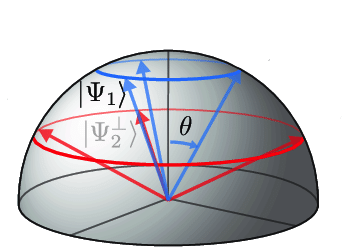
\includegraphics[width=0.5\textwidth]{assets/sphere}}

\ex{Exam 2017: Show that the following represents a sphere, and indicate its center and radius

$$x^2 + y^2 + z^2 + 2(x-4y+z) + 15 = 0$$ 

\par{By completing the square, we obtain the equation of the sphere in the canonical form, from where we can directly read the required data}

$$(x+1)^2 + (y-4)^2 + (z+1)^2 = 3$$

\par{Hence, $C(-1,4,-1) \quad r=\sqrt{3}$}
}

\newpage

\subsection{Line Equations}

\defn{Direction Vector}{any non-zero vector parallel to the line}

\par{We can define any point on a line, and hence define the line in general, by using the notion of component vectors seen above. Consider a line which passes through $A(\alpha, \beta, \lambda)$ and has direction vector $\vc{u} = (l,m,n)$, then the position vector of a random point $P(x,y,z)$ can be given by the sum of $\vc{a}$ with some multiple of $\vc{u}$; i.e. we can get to $P$ by first travelling from the origin until a point $A$ on the line and then travel \ita{along} the line}

\defn{Vector Form}{$$ \vc{p} = \vc{a} + t\vc{u}$$}

\par{By expanding the vector equation into its component form, we get two other representations of a line}

\defn{Parametric Form}{$$ (x,y,z) = (\alpha, \beta, \lambda) + t(l,m,n) = (\alpha + tl, \beta +tm, \lambda + tn)$$}

\defn{Symmetric Form}{$$ \frac { x - \alpha } { l } = \frac { y - \beta } { m } = \frac { z - \lambda } { n } = t$$}

\rem{Note that from the symmetric form one obtains directly the direction vector (denominator) and the coordinates of a point on the line (numerator)}

\subsection{Intersection of Lines}

\par{In $\real^3$, non-parallel lines need not intersect, they can be \ita{skew} ; varying their "z-index"/"height", shifts the plane they're in and they'll never meet. Hence, by equating two lines, we find}

\begin{itemize}
\item[] \textbf{Parallel} if their direction vectors are multiples of each other
\item[] \textbf{Intersect} if the system of equations given by equating their line equations is consistent
\item[] \textbf{Skew} if they are not parallel nor intersect
\end{itemize}

\subsection{Dot Product}



\lecture{18}{02}{2019}

\par{In order to find the dot product of two non-zero vectors $\vc{a}$ and $\vc{b}$ we split the vector $\vc{a}$ into two components: parallel $\vc{a}_{||}$ and perpendicular $\vc{a}_{\bot}$. In general: }

\prop{ }{$$ \vc{a} \cdot \vc{b} = a_{x}b_{x} + a_{y}b_{y} + a_{z}b_{z} $$}

\proofs{
\begin{align*}
	\vc{a} \cdot \vc{b} &= (a_{x}\vc{i} + a_{y}\vc{j} + a_{z}\vc{k}) \cdot (b_{x}\vc{i} + b_{y}\vc{j} + b_{z}\vc{k}) \\
	&=  \left( a _ { x } b _ { x } \right) ( \vc { i } \cdot \vc { i } ) + \left( a _ { y } b _ { y } \right) ( \vc { j } \cdot \vc { j } ) + \left( a _ { z } b _ { z } \right) ( \vc { k } \cdot \vc { k } ) \\ &+ \left( a _ { x } b _ { y } + a _ { y } b _ { x } \right) ( \vc { i } \cdot \vc { j } ) + \left( a _ { x } b _ { z } + a _ { z } b _ { x } \right) ( \vc { i } \cdot \vc { k } )  \\
	 &+ \left( a _ { y } b _ { z } + a _ { z } b _ { y } \right) ( \vc { j } \cdot \vc { k } ) \\
	&=  \left( a _ { x } b _ { x } \right) ( \vc { i } \cdot \vc { i } ) + \left( a _ { y } b _ { y } \right) ( \vc { j } \cdot \vc { j } ) + \left( a _ { z } b _ { z } \right) ( \vc { k } \cdot \vc { k } ) + 0 + 0 + 0^{*}  \\ 
	&=  \left( a _ { x } b _ { x } \right) | \vc { i } | ^ { 2 } + \left( a _ { y } b _ { y } \right) | \vc { j } | ^ { 2 } + \left( a _ { z } b _ { z } \right) | \vc { k } | ^ { 2 } \\ 
	&= \left( a _ { x } b _ { x } \right) + \left( a _ { y } b _ { y } \right) + \left( a _ { z } b _ { z } \right) 
\end{align*}	
}
\mymarginpar{*because $\bot$}

\subsection{Applications to geometry}

\subsubsection{Equations of planes}

\prop{}{ A plane $P$ with normal $(a,b,c)$ has equation: $ax + by + cz = d$}

\proofs{ Let $\vc{u} = (a,b,c)$ and $A(\alpha,\beta,\lambda) \quad B(x,y,z)$ be two points on $P$. Then by (\ref{plane:normal}),
\begin{align*}
&\vc{u} \cdot \overrightarrow{AB} = 0 \\
&(a,b,c) \cdot (x-\alpha, y-\beta, z-\lambda) = 0 \\
&a(x-\alpha) + b(y-\beta) + c(z-\lambda) = 0 \\
&ax + by + cz = \underbrace{a\alpha + b\beta + c\lambda}_{d}
\end{align*}
}
	
\ex{See 54 \#3.11}

\subsection{Angles}

\prop{}{There are two complimentary angles $(\alpha, \beta)$ between any two lines, which satisfy $\alpha + \beta = \pi$. These angles can be found by the dot product of their direction vectors}

\prop{}{Similarly, the angle between two planes is the angle between normal vectors for each plane}

\ex{Find the acute angle($\alpha$) between $P1 : x + 2y + 2z = 5 $ and $P2 : x - y - 4z = 6$ \\

\par{Normals: $\vc{u}=(1,2,2)$ and $\vc{v}=(1,-1,-4)$ . By the dot product we have that:}

\begin{align*}
\vc{u} \cdot \vc{v} &= |\vc{u}||\vc{v}|\cos(\theta) \\
\iff \cos(\theta) &= \frac{\vc{u} \cdot \vc{v}}{|\vc{u}||\vc{v}|} \\
\iff \cos(\theta) &= \frac{-9}{3\sqrt{18}} = -\frac{1}{\sqrt{2}} \\
&\implies \theta = \frac{3\pi}{4}
\end{align*}

\par{But since we were asked to find the \ita{acute} angle, we have that $\alpha = \frac{\pi}{4}$}
}

\lecture{19}{02}{2019}
\subsection{Projection of a point onto a plane and line}

\rem{Key insight is to realize that the projection ($B$) of the projected point ($A$) will be at the intersection of the line  $AB$ and the plane. This can be found by using the normal to the plane as the direction vector of the line $AB$, and equating the line and plane equations.}

\ex{ 55 \#3.13}

\rem{Similarly, to a line, all one needs to do is to find the intersection between the two perpendicular lines}

\subsection{Cross Product}

\prop{}{Let $\vc{a}$ and $\vc{b}$ be two non-zero vectors. Then, $$ \vc{a} \times \vc{v} = (a_yb_z - a_zb_y)\vc{i} + (a_xb_z - a_zb_x)\vc{j} +(a_xb_y - a_yb_x)\vc{k}$$}

\proof{Apply the distributive property, eliminate the product of perpendicular vectors ($=0$) and group like terms in terms of unit vectors}

\prop{Determinant Formula }{ Let $R1$ of a $3\times3$ matrix represent the standard unit vectors $\vc{i}, \vc{j}, \vc{k}$ , and $R2, R3$ represent the coordinates of $\vc{a} , \vc{b}$. Then, their cross product can be calculated by taking the determinant of the matrix
$$
\vc{a} \times \vc{b} =
\left|\begin{matrix}
\vc{i} &  \vc{j} & \vc{k}  \\
a_x &  a_y & a_z  \\
 b_x &  b_y & b_z \\
\end{matrix}\right|$$
}

\mymarginpar{TODO: applications}

\subsection{Applications}

\subsubsection{Area}

For $ \vc{u} = (u_x , u_y , u_z) \ , \ \vc{v} = (v_x , v_y , v_z)$ , the magnitude of the cross-product represents the area of the parallelogram $$Area = |\vc{u} \times \vc{v}|$$

\lecture{25}{02}{2019}

\subsection{Vector Triple Products}

\prop{Product Formula }{ For any vectors $\vc{u}, \vc{v}, \vc{w}$ $$ \vc{u} \times (\vc{v} \times \vc{w}) = (\vc{u} \cdot \vc{w})\vc{v} - (\vc{u} \cdot \vc{v})\vc{w}$$}

\subsection{Scalar Triple Products}

\nota{ $[\vc{u}, \vc{v} , \vc{w}]$}

\par{The STP of $\vc{u}, \vc{v} , \vc{w}$ (in that order) is given by $\vc{u} \cdot (\vc{v} \times \vc{w})$. Which is equal to the determinant of their $3\times3$ matrix}

\prop{STP }{ $$[\vc{u}, \vc{v} , \vc{w}] = \left|\begin{matrix}
u_x &  u_y & u_z  \\
v_x &  v_y & v_z  \\
 w_x &  w_y & w_z \\
\end{matrix}\right|$$
}

\proofs{ $$\vc{v} \times \vc{w} =
\left|\begin{matrix}
\vc{i} &  \vc{j} & \vc{k}  \\
v_x &  v_y & v_z  \\
 w_x &  w_y & w_z \\
\end{matrix}\right| = \left| \begin{array}{cc}{v_{y}} & {v_{z}} \\ {w_{y}} & {w_{z}}\end{array}\right| \mathbf{i}-\left| \begin{array}{cc}{v_{x}} & {v_{z}} \\ {w_{x}} & {w_{z}}\end{array}\right| \mathbf{j}+\left| \begin{array}{cc}{v_{x}} & {v_{y}} \\ {w_{x}} & {w_{y}}\end{array}\right| \mathbf{k}$$

Hence, 
$$
\begin{aligned} \mathrm{LHS} &=\mathbf{u} \cdot(\mathbf{v} \times \mathbf{w}) \\ &=u_{x} \left| \begin{array}{cc}{v_{y}} & {v_{z}} \\ {w_{y}} & {w_{z}}\end{array}\right|-u_{y} \left| \begin{array}{cc}{v_{x}} & {v_{z}} \\ {w_{x}} & {w_{z}}\end{array}\right|+u_{z} \left| \begin{array}{cc}{v_{x}} & {v_{y}} \\ {w_{x}} & {w_{y}}\end{array}\right| \\ &=\left|\begin{matrix}
u_x &  u_y & u_z  \\
v_x &  v_y & v_z  \\
 w_x &  w_y & w_z \\
\end{matrix}\right| = \mathrm{RHS} \end{aligned}
$$
}

\subsection{Coplanarity}

\defn{Coplanar}{4+ points are coplanar, if they lie on the same plane}


\prop{}{ Given 4 distinct points $O, U, V, W$, let $\vc{u} , \vc{v} , \vc{w}$ represent the coplanar position vectors from $O$, then $$[\vc{u},\vc{v},\vc{w}] = 0$$
}

\rem{If any two vectors are equal, then $[\vc{u},\vc{v},\vc{w}] = 0$}

\subsection{Symmetry}

\prop{}{ $$ [\vc{v},\vc{w},\vc{u}] =  [\vc{u},\vc{v},\vc{w}] =  [\vc{w},\vc{u},\vc{v}] \quad (1) $$ \\
and

$$  [\vc{v},\vc{u},\vc{w}] =  [\vc{w},\vc{v},\vc{u}] =  [\vc{u},\vc{w},\vc{v}] = - (1) $$
}

\proofs{It follows from the fact that interchanging two matrix rows, is equal to taking the symmetric of the original matrix , i.e.$$ \left| \begin{array}{lll}{a} & {b} & {c} \\ {p} & {q} & {r} \\ {x} & {y} & {z}\end{array}\right|=-\left| \begin{array}{lll}{p} & {q} & {r} \\ {a} & {b} & {c} \\ {x} & {y} & {z}\end{array}\right|$$}

\ex{Prove that $(\vc{a} \times \vc{b}) \times (\vc{a} \times \vc{c}) = [\vc{a}, \vc{b}, \vc{c}]\vc{a}$

$$\begin{aligned}(\mathbf{a} \times \mathbf{b}) \times(\mathbf{a} \times \mathbf{c}) &=((\mathbf{a} \times \mathbf{b}) \cdot \mathbf{c}) \mathbf{a}-((\mathbf{a} \times \mathbf{b}) \cdot \mathbf{a}) \mathbf{c} \\ &=(\mathbf{c} \cdot(\mathbf{a} \times \mathbf{b})) \mathbf{a}-(\mathbf{a} \cdot(\mathbf{a} \times \mathbf{b})) \mathbf{c} \\ &=[\mathbf{c} \cdot \mathbf{a}, \mathbf{b}] \mathbf{a}-[\mathbf{a}, \mathbf{a}, \mathbf{b}] \mathbf{c} \\ &=[\mathbf{c}, \mathbf{a}, \mathbf{b}] \mathbf{a}-0 \mathbf{c} \\ &=[\mathbf{a}, \mathbf{b}, \mathbf{c}] \mathbf{a} \end{aligned}$$
}
\newpage
\section{Logical Matters \& Proof}
\lecture{26}{02}{2019}
\defn{Direct Proof}{It consists of an argument that starts from the hypothesis and by a sequence of logical steps ends at the conclusion}

\rem{A common misconception is starting from the conclusion and finding something "true", by using both sides of the equation simultaneously}

\ex{Prove that the product of two odd integers is also odd}

\proofs{ Let $a, b$ be arbitrary odd integers. Then a $ a = 2k + 1$ and $b = 2l + 1$, for some $k, l \in \z$. Hence, \\

\begin{align*}
	ab &= (2k + 1)(2l + 1) \\
	&= 4kl + 2k + 2l + 1 \\
	&= 2(2kl + k + l) + 1
\end{align*}

Therefore, since $2kl + k + l \in \z$, $ab$ is odd.}


\subsection{\ita{if...then} \quad $\implies$}

\par{For any two propositions $p, q$ $p \implies q$ , reads \ita{ p implies q}. The truth values of the compound statement can be shown on a truth table. \\}

\begin{minipage}[c]{.5\textwidth}
	\begin{tabular}{|c|c|c|}
		$p$ & $q$ & $p \implies q$  \\
		\hline
		T & T & T \\
		T & F & F \\
		F & T & T \\
		F & F & T
	\end{tabular}
	\end{minipage}

\rem{Statements of this type show a truth \ita{relationship} between two statements, but say nothing about the truth value of the atomic propositions}

\par{The \ita{converse} of the above is $q \implies p$}

\begin{minipage}[c]{.5\textwidth}
	\begin{tabular}{|c|c|c|c|}
		$p$ & $q$ & $p \implies q$ & $q \implies p$ \\
		\hline
		T & T & T & T\\
		T & F & F & T\\
		F & T & T & F\\
		F & F & T & T 
	\end{tabular}
	\end{minipage}
	
\ex{ Let $ p = \text{\ita{x is a dog}}$ and $q = \text{\ita{x is a mammal}}$

$$ p \implies q = T \quad \quad q \implies p = F$$
}

\par{The negation of the atomic propositions is called the \ita{contrapositive}}

\rem{Contrapositive statements are equivalent}

$$\neg q \implies \neg \text{ p is the contrapositive of } p \implies q$$

\begin{minipage}[c]{.5\textwidth}
	\begin{tabular}{|c|c|c|c|c|c|}
		$p$ & $q$ & $\neg q$ & $\neg p$ & $\neg q \implies \neg p$ & $p \implies q$\\
		\hline
		T & T & F & F & T & T\\
		T & F & T & F & F & F\\
		F & T & F & T & T & T\\
		F & F & T & T & T & T
	\end{tabular}
\end{minipage}

\subsection{ \ita{if and only iff} , \ \ita{iff} , \ \ita{equivalent} , $\iff$}

\par{The compound statement is only true, if both atomic propositions have the same truth value. When carrying out a proof of this type, one usually splits the proof into two parts (1) $p \implies q$ (2) $q \implies p$ \\}

\begin{minipage}[c]{.5\textwidth}
	\begin{tabular}{|c|c|c|c|c|}
		$p$ & $q$ & $p \implies q$ & $q \implies p$ & $p \iff q$ \\
		\hline
		T & T & T & T & T\\
		T & F & F & T & F\\
		F & T & T & F & F\\
		F & F & T & T & T
	\end{tabular}
\end{minipage}
~\\
\ex{Prove that $ x^2 < 1 \iff -1 < x < 1$ \\

\par{(1) $p \implies q$ :$ \begin{array}{l}{\text { Suppose that } x^{2}<1 . \text { Then } x^{2}-1=(x+1)(x-1)<0 . \text { This }} \\ {\text { means that factors } x+1 \text { and } x-1 \text { have opposite signs and so }} \\ {\text { either }(x>-1 \text { and } x<1) \text { or }(x<-1 \text { and } x>1) . \text { The latter case }} \\ {\text { is impossible and so }-1<x<1, \text { as required. }}\end{array}$ }

\par{~\\(2) $q \implies p$ : $\begin{array}{l}{\text {Suppose that }-1<x<1 . \text { Then } x>-1 \text { and } x<1, \text { i.e. } x+1>0} \\ {\quad \text { and } x-1<0 . \text { Therefore } x^{2}-1=(x+1)(x-1)<0, \text { and hence }} \\ {x^{2}<1, \text { as required. }}\end{array}$}

\par{Hence, $ p \iff q$}
}

\lecture{04}{03}{2019}

\subsection{Proof by Contradiction}

\par{A proof by cotrandiction, or \ita{reductio ad absurdum}, relies on the simple logical necessity that for a given statement $P$ , either $P$ is true or $\not P$ is true, but given that we know the truth value of one, we can immediately deduce the other's. In particular, we assume $\not P$ to be true, and then work towards a contradiction}

\ex{ Given that $\sqrt{2}$ is know to be irrational, proof by contradiction that $\sqrt{2} - 1$ is also irrational}

\proofs{ We have the 2 following propositions: $$P_1 : \sqrt{2} \notin \q \quad \quad P_2 : \sqrt{2} + 1 \in \q $$
\par{Given that we know $P_1$ to be true, and assuming that $P_2$ is true. Then, it follows , by virtue of the fact that $\q$ is closed under subtraction, that $(\sqrt{2}+1) -1 \in \q$ , which in turn implies that $\sqrt{2} \in \q$. But, this contradicts $P_1$ which we \ita{know} to be true, hence $P_2$ is false , which means that $\neg P_2$ is true, i.e. 
$$ \neg P_2 = \neg(\sqrt{2} + 1 \in \q) = \sqrt{2} + 1 \notin \q $$ \quad \quad QED}}

\ex{Let A, B be $n \times n$ matrices. Show that if A is singular, then AB is also singular.}

\proofs{Let A be singular. Assume that AB is non-singular, with inverse Q satisfying (AB)Q = I. Using the associativity of matrix multiplication, A(BQ) = I and so A is non-singular (with inverse BQ). This is a contradiction of the hypothesis. It follows that AB must be singular.}

\subsection{Counterexample}

\par{Although, when trying to proof a statement it is necessary to find a general proof that covers all possible cases. To disprove it, one only needs to find a single case which does not satisfy it. We call this a \ita{counterexample}}

\ex{ The sum of two irrational numbers is irrational}
\proofs{ $\sqrt{2} + -\sqrt{2} = 0$ , 0 is not irrational, hence the statement is false}

\lecture{05}{03}{2019}

\subsection{Proof by Induction}

\defn{Induction Principle: }{let $P(n)$ be a statement which involves a natural number $n$; if (A) $P(1)$ is true and (B) $P(k) \implies P(k+ 1)$ for all natural numbers $k$, then $P(n)$ is true for all $n$}

\par{The goal here is to have a simple base case ($m$) which is easily shown to be true, then choose a random number ($k$) greater than $m$. Then, assuming that $P_k$ is true , and showing that $P_{k+1}$ is true , we also show that $P$ is true for any $k \geq m$.\mymarginpar{Useful to think of the domino effect}}

\begin{enumerate}
	\item Clearly identify and state $P$
	\item Check that $P_m$ is true 
	\item \ita{Inductive Hypothesis: } For arbitrary $k \geq m$, assume $P_k$ to be true * \mymarginpar{(*3) , (4) show that $P_k \implies P_{k+1}$ , for any $k\geq m$}
	\item From (3) , deduce that $P_{k+1}$ is true
\end{enumerate}
\newpage
\ex{Proof by induction the following: $$\sum_{i=1}^{n}{i^3} = \frac{1}{4}n^2(n+1)^2$$}

\proofs{

\begin{enumerate}
\item $P$ is the statement above
\item Checking that $P$ is true for $n=1$

$$\sum_{i=1}^{1}{1^3} = 1 = \frac{1}{4}1^2(1+1)^2$$

\item Inductive Hypothesis : we assume true for $n = k$, 

\item Using our assumption in (3), for $n = k+1$ we have that:

\begin{align*}
	\sum_{i=1}^{k+1}{i^3} &= \sum_{i=1}^{k}{i^3} + (k+1)^3 \\
		&= \frac{1}{4}\left(k^2(k+1)^2 + 4(k+1)^3\right) \\
		&= \frac{1}{4}\left((k+1)^2(k^2 + 4(k+1))\right) \\
		&= \frac{1}{4}\left((k+1)^2(k+2)^2\right) \\
		&= \frac{1}{4}n^2(n+1)^2
\end{align*}
\end{enumerate}

\par{Hence, it follows from the principle of induction that $P$ is true}
}

\newpage

\subsection{Inequalities*}
\mymarginpar{*EXTRA: Non-Examinable}

\newpage
\section{Complex Numbers}

\defn{Complex Polynomial}{ For a given complex number $\alpha$ $$f(\alpha)=a_{n} \alpha^{n}+a_{n-1} \alpha^{n-1}+\cdots+a_{2} \alpha^{2}+a_{1} \alpha+a_{0}$$}


\prop{}{If $a$ is a \textbf{non-real}, complex root of a real polynomial $f(x)$, then $a$ is a second root of $f(x)$}

\proofs{\par{From the complex conjugate's properties covered in 1R, we have that:} \mymarginpar{Given that $a_j \in \real \quad \overline{a_j} = a_j$ }
$$\begin{aligned} \overline{f(\alpha)} &=\overline{a_{n}}(\overline{\alpha})^{n}+\overline{a_{n-1}}(\overline{\alpha})^{n-1}+\cdots+\overline{a_{2}}(\overline{\alpha})^{2}+\overline{a_{1}} \overline{\alpha}+\overline{a}_{0} \\ &=a_{n}(\overline{\alpha})^{n}+a_{n-1}(\overline{\alpha})^{n-1}+\cdots+a_{2}(\overline{\alpha})^{2}+a_{1} \overline{\alpha}+a_{0} \\ &=f(\overline{\alpha}) \end{aligned}$$

\par{It follows, that if $f(\alpha)=0$ then $f(\overline{\alpha}) = \overline{0} = 0$. Hence, we can extrapolate the above proposition}}

\prop{}{$f(x)$ has real irreducible quadratic factor $$(x-\alpha)(x-\overline{\alpha}) = x^2 - 2xRe(\alpha) + |\alpha|^2$$, or in polar form , $$= x^2 - 2x\cos(\alpha) + r^2$$ \mymarginpar{Recall the polar form: $re^{i\theta} = r(\cos(\theta) + i\sin(\theta))$}}

\proofs{By the factor theorem, and from $(5.2)$, it follows that $f(x)$ has quadratic factor 

\begin{align*}
(x-\alpha)(x-\overline{\alpha}) &= x^2 - x\overline{\alpha} - x\alpha + \alpha\overline{\alpha} \\
	&= x^2 - x(\overline{\alpha} + \alpha) + (a^2 + b^2) \\
	&= x^2 - 2xRe(\alpha) + |\alpha|^2
\end{align*}
}

\theorem{}{Every real polynomial can be factorised as a product of real linear and real irreducible quadratic factors}

\proofs{}

\newpage
\nocite{*}
\printbibliography



\end{document}
